% --------------------------------------------------------------------------------

\begin{exercise}

Beweisen Sie Proposition $2.17$ aus dem Vorlesungsskript.

\end{exercise}

% --------------------------------------------------------------------------------

\begin{solution}

\phantom{}

\begin{figure}[h!]
    \centering
    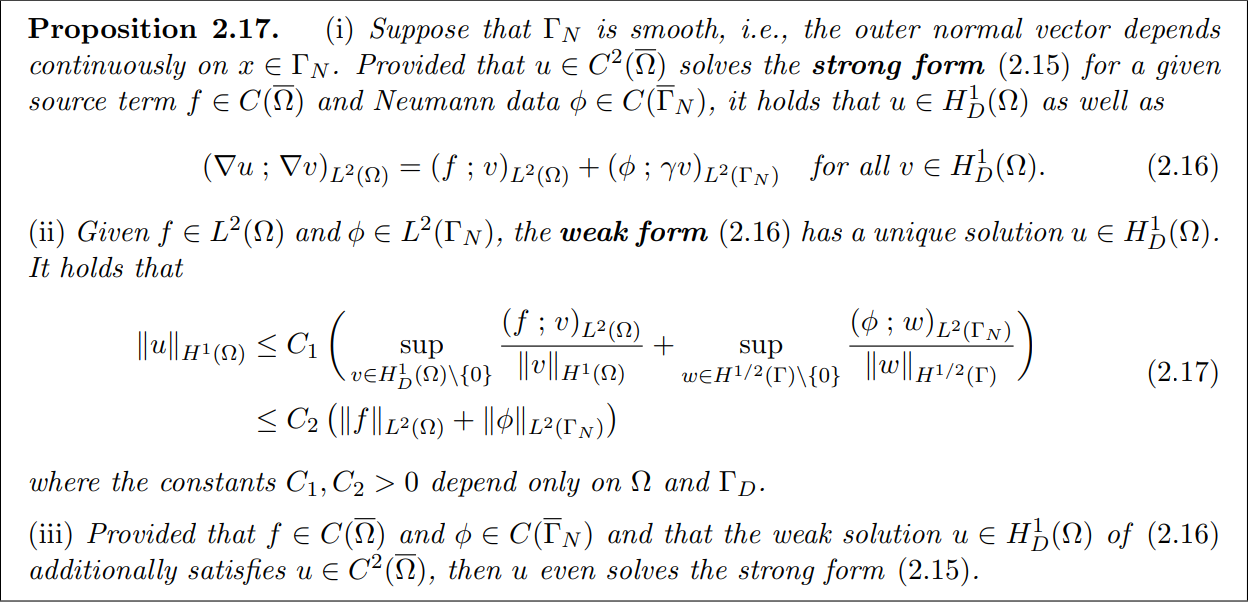
\includegraphics[width = 0.95 \textwidth]{Proposition 2.17.png}
\end{figure}

\begin{figure}[h!]
    \centering
    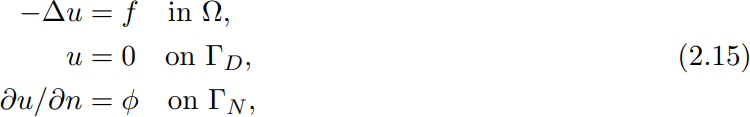
\includegraphics[width = 0.55 \textwidth]{(2.15).png}
\end{figure}

\begin{enumerate}[label = (\roman*)]

    \item $u \in C^2(\overline{\Omega})$ und $u = 0$ auf $\Gamma_D$.

    \begin{align*}
        \implies
        u
        \in
        \Bbraces{v \in C^1(\overline{\Omega}): v|_{\Gamma_D} = 0}
        =:
        C_D^1(\overline{\Omega})
        \subseteq
        \overline
        {
            C_D^1(\overline{\Omega})
        }^{
            \norm[H^1(\Omega)]{\cdot}
        }
        =:
        H^1_D(\Omega)
    \end{align*}

    \includegraphicsboxed
    [mehrdimensionales Analogon der partiellen Integration - Partielle Differentialgleichungen - Jüngel]
    [mAdpI-PD-J]
    {mehrdimensionales Analogon der partiellen Integration.png}

    Wir benutzen Partielle Integration, so wie in \ref{fig:mAdpI-PD-J}, mit $v$ und $\nabla u$ statt $u$ bzw. $F$.

    \begin{multline*}
        \implies
        \text{rhs}
        =
        \Int[\Omega]{f v}{x}
        +
        \Int[\Gamma_N]{\phi v}{s}
        =
        -\Int[\Omega]{(\Delta u) v}{x}
        +
        \Int[\Gamma_N]{\pderivative[][u]{\nu} v}{s}
        +
        \underbrace
        {
            \Int[\Gamma_D]{\pderivative[][u]{\nu} v}{s}
        }_0 \\
        =
        -\Int[\Omega]{\Div(\nabla u) v}{x}
        +
        \Int[\partial \Omega]{(\nabla u \cdot \nu) v}{s}
        \stackrel{\text{PI}}{=}
        \Int[\Omega]{\nabla u \cdot \nabla u}{x}
        =
        \text{lhs}
    \end{multline*}

    \item

    \begin{figure}[h!]
        \centering
        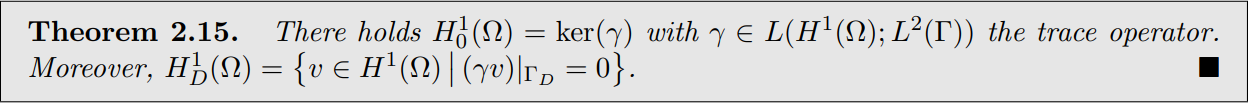
\includegraphics[width = 0.95 \textwidth]{Theorem 2.15.png}
    \end{figure}

    \begin{figure}[h!]
        \centering
        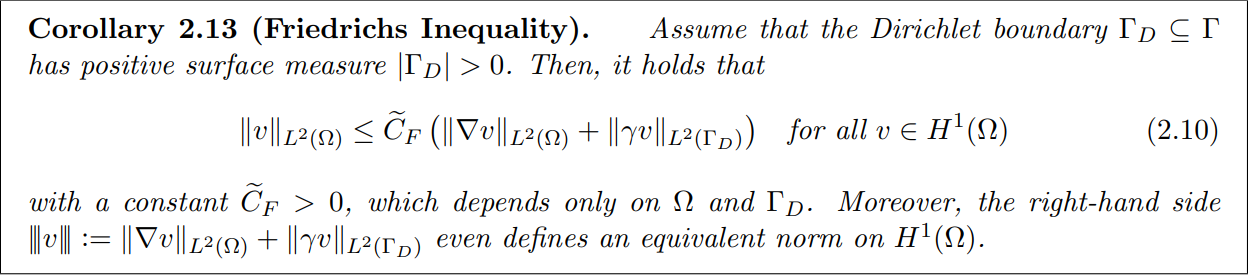
\includegraphics[width = 0.95 \textwidth]{Corollary 2.13 (Friedrichs Inequality).png}
    \end{figure}

    Laut Theorem 2.15 und Corollary 2.13 (Friedrichs Inequality), bildet die linke Seite von (2.16) ein Skalarprodukt (in $u$ und $v$) auf dem abgeschlossenen $H_D^1(\Omega)$.
    Wir erhalten also einen Hilbertraum.
    Die rechte Seite von (2.16) bildet ein lineares Funktional (in $v$).
    
    \begin{figure}[h!]
        \centering
        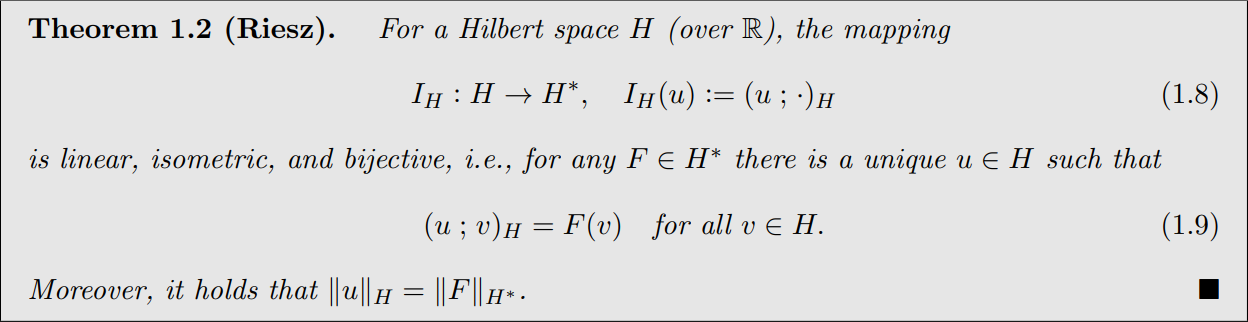
\includegraphics[width = 0.95 \textwidth]{Theorem 1.2 (Riesz).png}
    \end{figure}

    Laut Theorem 1.2 (Riesz), folgt daher die eindeutige Existenz einer Lösung $u \in H_D^1(\Omega)$ von (2.16).
    Wir erinnern uns nun an die Exercise 9 und den darin definierten Raum $H^{1/2}(\Gamma)$ mit seiner Norm $\norm[H^{1/2}(\Gamma)]{\cdot}$.

    \begin{figure}[h!]
        \centering
        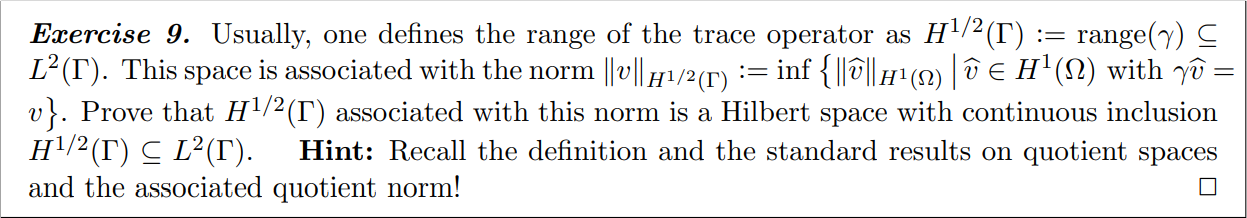
\includegraphics[width = 0.95 \textwidth]{Exercise 9.png}
    \end{figure}

    \begin{multline*}
        \implies
        \norm[L^1(\Omega)]{\nabla u}^2
        =
        (\nabla u; \nabla u)_{L^1(\Omega)}
        \stackrel{\text{(2.16)}}{=}
        (f; u)_{L^1(\Omega)}
        +
        (\phi; \gamma u)_{L^2(\Gamma_N)} \\
        \leq
        \sup_{v \in H_0^1(\Omega) \setminus \Bbraces{0}}
        \frac
        {
            (f; v)_{L^2(\Omega)}
        }{
            \norm[H^1(\Omega)]{v}
        }
        \norm[H^1(\Omega)]{u}
        +
        \sup_{w \in H^{1/2}(\Gamma) \setminus \Bbraces{0}}
        \frac
        {
            (\phi; w)_{L^2(\Gamma_N)}
        }{
            \norm[H^{1/2}(\Gamma)]{w}
        }
        \underbrace
        {
            \norm[H^{1/2}(\Gamma)]{\gamma u}
        }_{
            \leq
            \norm[H^1(\Omega)]{u}
        }
    \end{multline*}

    Mit Corollary 2.13 (Friedrichs Inequality), Cauchy-Schwarz-Bunjakowski, und der Stetigkeit (d.h. Beschränktheit) von $\gamma$ erhalten wir die gewünschten Ungleichungen.

    \begin{align*}
        \norm[H^1(\Omega)]{u}
        & \stackrel{\text{2.13}}{\leq}
        \widetilde{C}_F
        \pbraces
        {
            \sup_{v \in H_0^1(\Omega) \setminus \Bbraces{0}}
            \frac
            {
                (f; v)_{L^2(\Omega)}
            }{
                \norm[H^1(\Omega)]{v}
            }
            +
            \sup_{w \in H^{1/2}(\Gamma) \setminus \Bbraces{0}}
            \frac
            {
                (\phi; w)_{L^2(\Gamma_N)}
            }{
                \norm[H^{1/2}(\Gamma)]{w}
            }
        } \\
        & \stackrel{\text{CSB}}{\leq}
        \widetilde{C}_F
        \pbraces
        {
            \sup_{v \in H_0^1(\Omega) \setminus \Bbraces{0}}
            \frac
            {
                \norm[L^2(\Omega)]{f}
                \norm[L^2(\Omega)]{v}
            }{
                \norm[H^1(\Omega)]{v}
            }
            +
            \sup_{w \in H^{1/2}(\Gamma) \setminus \Bbraces{0}}
            \frac
            {
                \norm[L^2(\Gamma_N)]{\phi}
                \norm[L^2(\Gamma_N)]{w}
            }{
                \norm[H^{1/2}(\Gamma)]{w}
            }
        } \\
        & =
        \widetilde{C}_F
        \Bigg (
            \norm[L^2(\Omega)]{f}
            \underbrace
            {
                \sup_{v \in H_0^1(\Omega) \setminus \Bbraces{0}}
                \frac
                {
                    \norm[L^2(\Omega)]{v}
                }{
                    \norm[H^1(\Omega)]{v}
                }
            }_{
                \leq 1
            }
            +
            \norm[L^2(\Gamma_N)]{\phi}
            \underbrace
            {
                \sup_{w \in H^{1/2}(\Gamma) \setminus \Bbraces{0}}
                \frac
                {
                    \norm[L^2(\Gamma_N)]{w}
                }{
                    \norm[H^{1/2}(\Gamma)]{w}
                }
            }_{
                =
                \norm{\gamma}
                <
                \infty
            }
        \Bigg ) \\
        & \leq
        \pbraces
        {
            \widetilde{C}_F
            \max \Bbraces{1, \norm{\gamma}}
        }
        \pbraces
        {
            \norm[L^2(\Omega)]{f}
            +
            \norm[L^2(\Gamma_N)]{\phi}
        }
    \end{align*}

\end{enumerate}

\end{solution}

% --------------------------------------------------------------------------------
